%%%%%%%%%%%%%%%%%%%%%%%%%%%%%%%%%%%%%%%%%%%%%%%%%%%%%%%%%%%%%%%%%%%%%%%%%%%%%%%%
%2345678901234567890123456789012345678901234567890123456789012345678901234567890
%        1         2         3         4         5         6         7         8
% DOCUMENT CLASS
\documentclass[oneside,12pt]{Classes/RoboticsLaTeX}

% USEFUL PACKAGES
% Commonly-used packages are included by default.
% Refer to section "Book - Useful packages" in the class file "Classes/RoboticsLaTeX.cls" for the complete list.
\usepackage{amsmath}
\usepackage{amsfonts}
\usepackage{algorithm}
\usepackage{algorithmic}
\usepackage{multirow}
\usepackage{colortbl}
\usepackage{color}
\usepackage[table]{xcolor}
\usepackage{epigraph}
\usepackage{graphicx}
\usepackage{subfigure}
\usepackage{caption}
%\usepackage{subcaption}
\usepackage{hyperref}
\usepackage{tabularx}
\usepackage{float}
\usepackage{longtable}
\usepackage[pdftex]{graphicx}
\usepackage{pdfpages}
\usepackage{tabularx}
\usepackage{pdflscape}
\usepackage[acronym,toc]{glossaries}
\usepackage{setspace}
\usepackage[utf8]{inputenc}
\usepackage[table]{xcolor}

\usepackage{emerald}
\usepackage{soul}
\usepackage{makecell}
\usepackage{booktabs}
\usepackage{adjustbox}

\setstretch{1.5}
%\onehalfspacing
% SPECIAL COMMANDS
% correct bad hyphenation
\hyphenation{op-tical net-works semi-conduc-tor}
\hyphenation{par-ti-cu-lar mo-du-le ge-stu-re}
% INTERLINEA 1.5
%\renewcommand{\baselinestretch}{1.5}

%% ignore slightly overfull and underfull boxes
%\hbadness=10000
%\hfuzz=50pt
% declare commonly used operators
%\DeclareMathOperator*{\argmax}{argmax}
%\ word count -> texcount Thesis_Eoghan.tex -inc -incbib -sum -1


% HEADER
\title{\Large{An Investigation into Biased Language in the American Sport Industry}}

  \author{Eoghan Ó Gallchóir (16339936)}
  \collegeordept{School of Computer Science}
  \university{National University of Ireland, Galway}
  \crest{
\includegraphics[width=75mm]{Figures/logo_NUI.png}}
  

% Supervisors
\supervisor{Dr. Peter Paul Buitelaar, \ Dr. Mihael Arcan}
%\supervisor{Dr. Mihael Arcan}	


% text before "In partial fulfillment of the requirements for the degree of" in .cls file/line 153\
% replace PROGRAMME with Data Analytics, Artificial Intelligence, or Artificial Intelligence - Online
\degree{MSc in Artificial Intelligence}
\degreedate{August 26, 2021}

%%%%%%%%%%%%%%%%%%%%%%%%%%%%%%%%%%%%%%%%%%%%%%%%%%%%%%%%%%%%%%%%%%%%%%%%%%%%%%%%
%%% uncomment if glossary needed, see examples in file
%\makeglossaries
%\loadglsentries{glossary}

\begin{document}
\begin{spacing}{1}
\maketitle
\end{spacing}

% add an empty page after title page
\newpage\null\thispagestyle{empty}\newpage

% set the number of sectioning levels that get number and appear in the contents
\setcounter{secnumdepth}{3}
\setcounter{tocdepth}{3}

\frontmatter

% replace PROGRAMME with Data Analytics, Artificial Intelligence, or Artificial Intelligence - Online
\textbf{DECLARATION} 

I, Eoghan Ó Gallchóir, do hereby declare that this thesis entitled {\it An Investigation into Biased Language in the American Sport Industry},
 is a bonafide record of research work done by me for the award of MSc in Artificial Intelligence from National University of Ireland, Galway. 
 It has not been previously submitted, in part or whole, to any university or institution for any degree, diploma, or other qualification. 
\newline

\begin{tabular}{@{}p{4in}p{4in}@{}}
Signature: {\ECFJD~~Eoghan Ó Gallchóir~~}
\end{tabular}
\newpage


%%%% uncomment if acknowledgements needed
%\textbf{Acknowledgement}
%
%
%\newpage\textbf{}


% THESIS ABSTRACT
\begin{abstracts}
%The abstract should summarize the substantive results of the work and not merely list topics to be discussed. An abstract is an outline/brief summary of your paper and your whole project ... 
To do after results have been determined
%It should be terse and usually written in the present tense and impersonal style: "A new graph community detection algorithm is proposed based on spectral features. It is compared against several strong baselines ...".

\textbf{Keywords: } Machine Learning, Natural Language Processing, Harvard General Inquirer, Sentiment Analysis, Text Classification
\end{abstracts}


\tableofcontents
\listoffigures
\listoftables
\printglossary[title=List of Acronyms,type=\acronymtype]

\mainmatter

\chapter{Introduction}
\label{chap:introduction}
\setcounter{page}{7}
The work carried out in this project involves classifying sentiment towards white and non-white
American football players. This is done through machine learning models.

\section{Background}
When players first enter any of the 4 major American sports (baseball, basketball, football and hockey) they are
drafted from colleges (or overseas) rather than signed or brought up from youth squads as commonly seen in
European sports like soccer or rugby. The National Football League (NFL) draft consists of 7 rounds, with each team
having 1 pick per round. With 32 teams in the league, that is a total of 224 selections to be made. Teams choose players in order based on performance, with worse performing teams 
receiving a higher pick in the draft. This is seen as a way to increase the competitiveness in the league, theoritically the worse the 
team is, the higher selection they have so they will get a better player. Also, the team with the 1st pick in the first round (no.1 overall), also 
receive the 1st pick in the second round (no.33 overall), and so on and on. It is however extremely difficult to evaluate college-level players,
for example 45\% of quarterbacks taken in the first round of the NFL draft were no longer on a team 5 years after they were drafted \footnote{\url{https://football.pitcherlist.com/pessimists-guide-to-the-nfl-draft/}}.
Currently there are 350 Division 1 universities in America \footnote{\url{https://www.ncaa.org/about/division-i-schools}}, this status
essentially describes the standard their sports programmes are at, Division 1 being the highest. This is where most
NFL players come from. Due to this size, it is unrealistic to expect that every NFL coach can assess every player of
interest to him to draft onto his team, so teams rely on scouting reports, from scouts they either hire or trust, to
help inform them in deciding on who to draft. These scouting reports describes a players physical and cognitive
attributes in the form of a short paragraph, also describing his strengths and weaknesses. An example of these strength and weaknesses can be seen in \hyperref[fig:bateman_s]{Figure 1.1} and \hyperref[fig:bateman_w]{Figure 1.2}. 
Most prospective players also attend a draft combine, which essentially is a standardized workout and assessment used to quantify their abilities. American sports media also produces
similar player analysis \footnote{\url{https://nfldraft.theringer.com/mock-draft}}, as well as game previews and post-game reports.

\begin{figure}[hb]
  \centering
  \begin{minipage}{.5\textwidth}
    \centering
    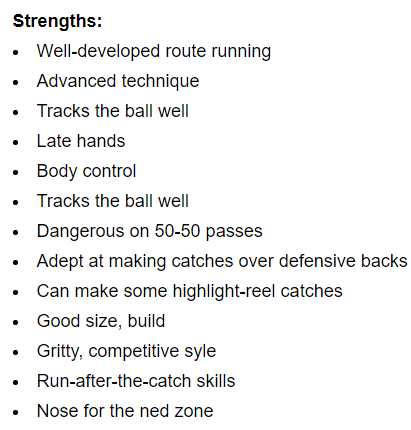
\includegraphics[width=.8\linewidth]{Figures/Bateman_Strengths.png}
    \captionof{figure}{Example of a players strengths}
    \label{fig:bateman_s}
  \end{minipage}%
  \begin{minipage}{.5\textwidth}
    \centering
    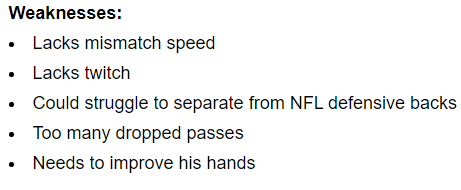
\includegraphics[width=.8\linewidth]{Figures/Bateman_Weaknesses.png}
    \captionof{figure}{Example of a players weaknesses}
    \label{fig:bateman_w}
  \end{minipage}
  \end{figure}

\section{Context}
Studies done on the American sports industry and its media has been time and time again shown that racism exists in sports media. One study by \citet{Viklund2009}
showed that racial bias still exists in NFL commentary, with the problem persisting across serveral different television network coverages.
The NFL is in a unique position for analysis as there is a huge
discrepancy in both players of colour and people of colour not only in team coaching and executive positions \footnote{\url{https://bit.ly/3gxzsEu}}, but in
reporting roles in mainstream media \footnote{\url{https://bit.ly/3mvzsbI}}. In the 2020/2021 season of the NFL, players of colour accounted for 69.4\% of 
all players, while there were only 4 head coaches of colour in the league in that same season (12.5\% of all head coaches). Similarily, it was found that 85\% 
of sports editors were white, and 80.3\% and 82.1\% of columnists and reporters were white, respectively.

\begin{figure}[hb]
  \centering
  \begin{minipage}{1\textwidth}
    \centering
    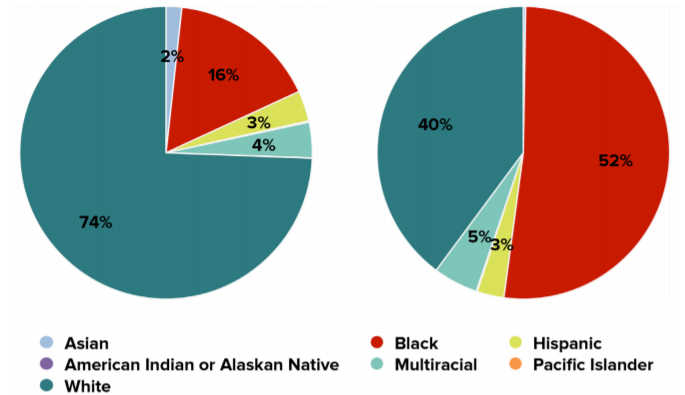
\includegraphics[width=1\linewidth]{Figures/Female_Enrolled_v_Disciplined.png}
    \captionof{figure}{Comparison of Racial Representation Among Enrolled Vs. Disciplined Females}
    \label{fig:Female_Rep}
  \end{minipage}%
\end{figure}


\section{Bias}
\subsection{Implicit Bias}
Implicit bias has been described by \citet{imp_bias} as attitudes that subconsciously affect our actions and decisions. These attitudes can be either
positive or negative, and are activated unintentionally. This is the opposit of explicit(or conscious) bias, where attitudes are intentionally affecting our
actions. Given how implicit bias is present in every one of us, it can take many different forms in many different areas of life. For example in education, 
a study \footnote{\url{http://kirwaninstitute.osu.edu/implicit-bias-training/resources/race-matters.pdf}} examined the rates of disciplinary actions in the 
Ohio education system faced not only by students of different races but also compared those rates on a per gender basis. It was found that:
\begin{itemize}
  \item black students received a disproportionate amount of discipline compared to their percentage of enrollment.
  \item black female students experienced the highest level of overrepresentation.
\end{itemize}
This clearly shows how prevalent and damaging bias can be. The study's results can be seen in \hyperref[fig:Female_Rep]{Figure 1.3}.
\subsection{Bias in Media}
Media has long played a role in shaping how some people view minority groups and race at large \citep{Greenberg2002Minorities}.
\citet{mediastudy} found the existence of both gender and racial stereotyping on television. Viewing women and minority
through this lens provides those who watch with conventional idealogical views about them \citep{mediastudy}. This study used code
to gather network televsion data over a period of nine years. The same coding schemes, and validity testing was used year-on-year. 
This study is relevant not only because of its subject matter but also due to its aforementioned methodology. The paper does however
fall short in several categories.
\begin{itemize}
  \item No popular paid channels like HBO were tracked during this time.
  \item The coders who implemented the research were only given a few weeks of training. Could lead to inconsistencies too as a different group oversaw each year.
\end{itemize}
With television being some peoples only interaction with ethnic groups outside their own, some authors have examined the effect that this stereotyping has on those who consume these programmes. 
As long as mainstream media continues to reproduce racial and ethnic stereotypes, these false characteristics will continue to exist, and viewers will see it as 
how people truly are \citep{Castaneda}.


\section{Thesis Structure}
This thesis is divided into seven chapters.
\begin{itemize}
  \item Chapter 1 provides background information and puts the investigation into context.
  \item Chapter 2 reviews current work in this domain, as well as literature review of papers on media bias, classification algoritms, and sentiment analysis techniques.
  \item Chapter 3 is a detailed look at the methods used to both analyse player sentiment and classify player ethicity.
  \item Chapter 4 describes the data created for and during the experiments.
  \item Chapter 5 details the experimental settings.
  \item Chapter 6 provides experiment results and interpretation.
  \item Chapter 7 gives a final review of the results in the context of the aim of this paper.
\end{itemize}


\chapter{Literature Review}
\label{chap:lit_review}
This chapter covers existing literature that relate to the core topics of this thesis.
\section{Sentiment Analysis}
\subsection{Basic Classification}
Sentiment analysis is the process in which the attitude or emotion expressed by a text is classified. This is done through natural language processing techniques. The rise of social media applications, Twitter in particular, 
has only increased interest in sentiment analysis. As NFL scouting reports are subjective, opinion-based documents, it is important to understand current classification methods of textual reviews. Experiments conducted by 
\citet{SentiAnalysis} showed that sentiment analysis of textual (in their case movie reviews) reviews could be classified at a document level. The research conducted does prove that large scale sentiment analysis of documents can
produce concrete results due to its use of the Cornell movie-review corpora. However, documents were not classified beyond positive and negative sentiment. While this binary classification is somewhat useful,
no specific information can be obtained from this, which is why Inquirer dictionaries shall be utilised in experiments conducted in later chapters of this paper.

\subsection{Using an Inquirer Dictionary}
Inquirer dictionaries are essentially tools to map words to dictionary-supplied categories. The General Inquirer (GI) dictionary is the most widely used in semantic analysis research, containing over 182 categories in all \citep{stone66}, 
far surpassing simple positive or negative sentiment that we have seen before. Currently, this dictionary is a combination of the Harvard IV-4, the Lasswell dictionaries, as well as contributions based on the social cognition work of 
Semin and Fiedler. A study by \citet{SentiGI} uses this GI dictionary to perform computer-assisted semantic analysis on product reviews on consumer opinion web sites. Outside of the positive and negative tags, 11 categories 
were found relevant to their research. Pollach's findings corroborated earlier experiments pertaining to word frequencies, causing them to conclude that these product reviews follow ``implicit genre rules regarding content, format 
and language''. This analysis shows that using an Inquirer dictionary yields results beyond simple positive or negative sentiment. It is also highly relevant because of the specificity of the corpus it analyses. The scope of the corpus analysed
in the Experiments chapter of this paper will have a similar corpus scope, and it is promising that multiple Inquirer categories were still discovered. A similar or higher number of categories should be found in the subject of NFL scouting reports.

\section{Text Classification with Machine Learning Algorithms}
Text classification is one of the core topics of this paper, and shall be the subject of one of the experiments performed in the experiments chapter. \citet{Chinese_textC} showed that the Support Vector Machine (SVM) algorithm was the most accurate for 
multi-label classification, albeit only slightly more accurate than the much quicker Naive Bayes (NB) algorithm. Due to this the SVM algorithm is only seen as appropriate for use with smaller datasets. The experiment is relevant to this paper due to the fact
that both the SVM algorithm and Naive Bayesian algorithm was implemented by the scikit-learn package and produced desirable results. More information on scikit-learn can be found in \hyperref[sec:sci-kit_label]{section 3.3}. Another one of its strengths
is the use of precision and recall in addition to the F1-score. This gives context to the F1-score. A weakness of this paper is that the smaller classes have better results than the big classes, which would lead to a reducution in expected accuracy under
practical circumstances.
\paragraph{}
\citet{Dharmadhikari2011EmpiricalSO} also posited that SVM is one of the most effective text classification algorithms due to its ability to manage large spaces of features. The two papers also agree its unwieldy comptuational 
demands.The papers findings also takes into account NLP techniques and how it can be used to improve classification results. A major weakness of this paper is the lack of experiments showing its findings, focusing entirely on existing literature. Another
algorithm that can be used for text classification is Stochastic Gradient Descent (SGD). It performs well with sparse and high dimensional data \citep{SVM_SGD}. \citet{Arabic_SGD_LR} found that on large, multi-label datasets, both SGD and Logistic Regression
had the highest F1-score in comparison to SVM and NB approaches.

\section{Dataset Imbalance}
Data imbalance occurs in many real world domains. Given that 70\% of NFL players are non-white, this applies to the problem domain of this paper. \citet{imbalanced_data} shows that imbalanced data affects the performance of normal classification, with balanced 
datasets achieving a higher average F1-score. It was found that the difference in classification performance between balanced and imbalanced data grew as the degree of imbalance distribution grew. One weakness of the experiments by \citet{imbalanced_data} 
is that it did not involve any text classification, something that is a core component of the experiments proposed in later in this paper. Oversampling the minority class, especially in datasets with a large discrepancy provided good results \citep{BalancingMethods}.
Furthermore, \citet{BalancingMethods} also found that random over-sampling was less computationally expensive than other methods to balance datasets. 

\section{Existing Work on Sports Media}
American sports, with American Football and the National Basketball League (NBA) specifically, are in a unique position, with the majority
of their players being non-white but other positions, beit coaching positions, executive positions or media positions being of a white majority \footnote{\url{https://bit.ly/3gxzsEu}}.
This has caused the two sports to be scrutinized more than most for bias in their respective media.
Studies have been conducted into the language used by television announcers or commentators. They give play-by-play description of what is happening at any given
time during the game. More often than not they are paired with an analyst, whose role is to provide expert analysis and background information about a player or team. 
An article by \citep{ColorCoded} analysed comments made by both the play-by-play commentator and the commentator tasked with analysis in American Football and Basketball collegiate games.
To sample the American Football it took only a quarter of each game over a period of weeks as their data sampling method.
For the basketball it used a Division 1 Men's Championship basketball tournament, obtaining over 55 hours of basketball coverage. 
They hypothesized that black players would receive:
\begin{itemize}
  \item a higher portion of negative comments than white players.
  \item more comments on their physical attributes than white players.
  \item more negative comments regarding both their intellect on and off the field.
  \item both more negative statements about their character and would recieve more negative personal interest stories than their white counterparts.
\end{itemize}
In each case the hypothesis was supported by their experiments.
This article's strength lies in how thorough it is despite its small sample size. The study would have however benefitted from a larger dataset, perhaps over
several years. In this paper it has been established the effect this implicit bias can have on viewers, discussion which is missing from \citet{ColorCoded}'s article.
\paragraph{}
There are instances of overcoming the problem of a small dataset. It was shown by \citep{CommentatorBias} that large scale analysis of American sports media was not only possble, 
but produced coherent results. 1,445 American football (both collegiate and NFL) games were automatically annotated with mentions of players and linked with metadata. To reduce
susceptibility to noise ARK TweetNLP was used as it is more robust than conventional part-of-speech tagging methods. One of the outputs of this study was their {\it FOOTBALL} dataset,
a large scale sports commentary corpus annotated with the race of the player, which is useful for any future work in bias of American football media. This paper is included here due to its
sound technical foundations, and how it is possible to produce definitive results from processing the language associated with sport. It also only furthers the need to analyse
scouting in this manner.



\chapter{Methodology}
\label{chap:methodology}
In this chapter, the method of sourcing the data is described. The classification and sentiment analysis experiments are also explained here ahead of their use in \hyperref[chap:experiments]{Chapter 5}.
\section{Data Gathering}
The data needed to perform the experiments proposed was not available from any resource online. Thus, web scraping techniques had to be implemented. It was decided upon that player data should
be obtained from the official NFL.com website \footnote{\url{https://www.nfl.com/draft/tracker/picks?year=2021}}. Beautiful Soup \footnote{\url{https://beautiful-soup-4.readthedocs.io/en/latest/}} (BS)
was used to obtain all player information from the most recent (2021) draft. Here is where the player in-depth profile URL link was also captured, which will also be parsed to find information to
make up the scouting report column of the datasets. As the web page in question uses Javascript to load its content, Chromium and Selenium was used to connect to the web page and allow the content to load before obtaining the information
needed to create the datasets. The page's Javascript loaded every player name, player position and player profile URL link under the same CSS tag, allowing for functions to iteratively grab the data. Part of the web page
can be seen in \hyperref[fig:NFL_draft]{Figure 3.1}.
The player scouting report was was obtained in a similar manner, using the aforementioned URL link with BS to get the player strength and weaknesses. The final column of the dataset, player race, 
was manually added, as there is no record of it on the web pages parsed. Each row in the dataset consists of many sentences pertaining to one player. To test the the different machine learning algorithms 
on how much information they need, the master dataset was split into 1-sentence, 2-sentence, and 5-sentence datasets. For more information on all the datasets created, see \hyperref[sec:class_data]{Chapter 4}.

\begin{figure}[hb]
  \centering
  \begin{minipage}{1\textwidth}
    \centering
    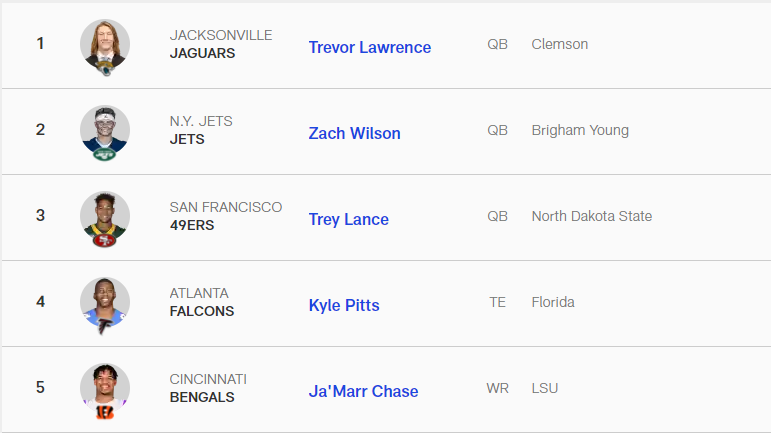
\includegraphics[width=1\linewidth]{Figures/NFLcom_example.png}
    \captionof{figure}{NFL.com's 2021 draft table}
    \label{fig:NFL_draft}
  \end{minipage}%
\end{figure}

\section{Using the Harvard General Inquirer to produce data}
\label{sec:GI_dict}
The Harvard General Inquirer dictionary is available to download for use from the harvard.edu website \footnote{\url{http://www.wjh.harvard.edu/~inquirer/spreadsheet_guide.htm}}. Using this file, a Python
dictionary of key-value pairs was created, the key being a stemmed word from the GI dictionary file and the values being each sentiment associated with it. With this dictionary, new datasets were created by 
applying the dictionary to the datasets created in the section above. This created a GI tagged version of the 1-sentence, 2-sentence, 5-sentence, and master dataset. The 1 sentence GI tagged 
dataset is what shall be used to perform the sentiment analysis experiment described later in the chapter.
The Harvard GI dictionary was also used to created an integer tagged version of the 1-sentence, 2-sentence, 5-sentence and master dataset. The dataset(s) columns were every GI tag found in the master dataset and 
the players ethnicity. Each row contained either a 1, indicating the gi tag was present in some sentence, or a 0, to indicate no presence of the tag. This was done in an attempt to improve the accuracy and f1-score Of
the GI tagged version of the aforementioned datasets. This collection of datasets shall be henceforth referred to as the binary-GI tagged group of datasets.

\section{Classification}
\label{sec:sci-kit_label}
This section decribes what machine learning tools were used to implement the classification experiment. The experiment's aim is to use different algorithms on the different datasets created to try and to
correctly classify between white and non-white instances. From this we can see what level of accuracy we can achieve, a higher score insinuating that language used can separate players by their ethnicity.
FLOWCHART
\subsection{Pre-processing}
Text pre-processing was performed on the scouting report sentences in each dataset before this experiment was performed.
Specifically:
\begin{itemize}
  \item stopword removal with the Natural Language Toolkit (NLTK) library.
  \item removal of any punctuation with NLTK.
  \item the stemming of words also with NLTK.
\end{itemize}
After this pre-processing, each report instance was then converted to a matrix of token counts through vectorization.

\subsection{Data Imbalance}
The data imbalance in the datasets in this thesis was rectified through oversampling of the minority, in this case white player, class. To do this, the \texttt{imbalanced-learn} libary \citep{imb-learn} is used.
Imbalanced-learn is an MIT-licensed library that uses scikit-learn that provided tools to deal with imbalanced classes during classification problems. It is an open source library that has
both under-sampling and over-sampling methods. It is also fully compatible with scikit-learn features. In this experiment, an imbalanced-learn pipeline was used. Over-sampling was implemented to oversample
the minority class and thus even the dataset.

\subsection{Algorithms}
To explore how many sentences are needed to produce the most accurate result, different ML algorithms were used. All algorithms were implemented with scikit-learn \citep{scikit-learn} 
due to its accessibility. It has a huge library of classification, regression, and clustering algorithms. The four algorithms used are:
\begin{itemize}
  \item {\it Logistic Regression}: In the case of this experiment, this classifier models the probability whether a scouting sentence(s) instance is either a white player or a non-white player.
  \item {\it Naive Bayes}: This is a simple classifier that assumes strong independence between features. However in this experiment, models are created on one feature, the scouting report sentence(s).
  \item {\it Stochastic Gradient Descent}: This algorithm works well for text classification due to the sparse nature of text classification \citep{SVM_SGD}.
  \item {\it Support Vector Machine}: Similar to SGD, SVM also works well for text classification.
\end{itemize}
Each of these algorithms were applied to all datasets created for classification. For details of the settings for each of these algorithms, see the chapter on \hyperref[chap:experiments]{experiment settings}.

\subsection{Evaluation}
Due to the fact that the data collected was small (\hyperref[chap:data]{see Data chapter}), evaluation techniques are used to combat this. 10-fold cross-validation was used over hold-out validation
as {\it k}-fold cross-validation produces more accuracte results \citep{k-fold_cross}. F1-scores are implemented as part of the accuracy evaluator. It was chosen over accuracy due to how important
precision and recall are in ML problems. The average F1-score was taken from the output of the {\it k}-fold cross-validation to produce results for each algorithm.

\section{Sentiment Analysis}
The second experiment proposed in this paper is to perform sentiment analysis on sentences cateogized by the Harvard GI. This include the Harvard IV-4 dicitonary and the Lasswell value dictionary.
The 1-sentence dataset shall be tagged with the sentence's GI category and the players race that the sentence pertains to. There are several steps involved in this method, described below.
FLOWCHART
\subsection{Obtaining all GI Tags}
Firstly, the aforementioned \hyperref[sec:GI_dict]{GI Python dictionary} of key-value pairs is used. A dataset is then parsed through and each key occurence for both white and non-white player reports
causes its value (its sentiment) to be kept track of. It is important to note that one word can have multiple GI tags. For example, {\it Confident} has 7 unique GI tags associated with it:
\begin{itemize}
  \item Positive - Positive words.
  \item Strong - Words implying strength.
  \item Power - Subset of strong, indicating a concern with power, control, or authority.
  \item Pleasure - Words indicating the enjoyment of a feeling, including words indicating confidence, interest, and commitment.
  \item EMOT - Words related to emotion.
  \item Ovrst - "Overstated", Words indicating emphasis in realms of speed, frequency, causality, inclusiveness, quantity or 
                  quasi-quantity, accuracy, validity, scope, size, clarity, exceptionality, intensity, likelihood, certainty and extremity.
  \item WlbTot - Words in well-being, relating to the health and safety of the player.
\end{itemize}
For each of these GI tags in both ethnicities, the percentage of their occurence was then calculated, and these figures were made into a dataset.
\subsection{Tagging the dataset}
From the dataset created above, GI tags deemed irrelevant were removed from the dataset. Using this dataset, the 1-sentence dataset, and the GI python dictionary, every row in the 1-sentence dataset was parsed through and all GI 
sentiments for that sentence was found and added to a new dataset, consisting of the player sentence, the GI tag, and player ethnicity. With this new data, the sentiment for each GI tag for both white and non-white players can be found,
as well as the difference between them. For more information on all datasets created for sentiment analysis see \hyperref[sec:senti_data]{Chapter 4}.

\chapter{Data}
\label{chap:data}
This chapter describes all data gathered for the purpose of experimentation.
\section{Classification Data}
\label{sec:class_data}
For the classification experiment, 4 different datasets were created. As mentioned in the \hyperref[chap:methodology]{Methodology chapter}, each dataset has a standardized structure. Column names of:
\begin{itemize}
  \item Player ID - Given to provide player anonymity, each player has their own unique identifier number. This becomes important in the 1-sentence, 2-sentence, and 5-sentence datasets because as the data becomes more divided, player sentences can
        still be grouped by their ID.
  \item Postion - Abbreviated player position. In this data, 17 player positions arose: \begin{itemize}
    \item C - Center.
    \item CB - Cornerback.
    \item DE - Defensive End.
    \item DT - Defensive Tackle.
    \item EDGE - Edgerusher.
    \item FB - Fullback.
    \item G- Guard.
    \item K - Kicker.
    \item LB - Linebacker.
    \item LS - Long Snapper.
    \item OT - Offensive Tackle.
    \item P - Punter.
    \item QB - Quarterback.
    \item RB - Running Back.
    \item SAF - Safety.
    \item TE - Tight End.
    \item WR - Wide Receiver.
  \end{itemize}
  \item Scouting Report Sentence(s) - These are sentences taken from a players strength and weaknesses list as described on NFL.com.
  \item Player Race - player race is denoted as either \textbf{W} - White or \textbf{NW} - Non-White.
\end{itemize}

\subsection{All Sentence Dataset}
This is the first dataset that was obtained, and is refered to in this paper as the master dataset. All other datasets pertaining to the classification experiment is derived from it. It contains:
\begin{itemize}
  \item 259 player rows in the format discussed above.
  \item Each player has an average of 17 sentences in their report. Player ID 1 has the most sentences at 31, player ID 225 has the least sentences associated with them at 4.
  \item Of the 259 players, 213 have been classified as NW and 46 have been classed as W.
\end{itemize}

\begin{figure}[hb]
  \centering
  \begin{minipage}{1\textwidth}
    \centering
    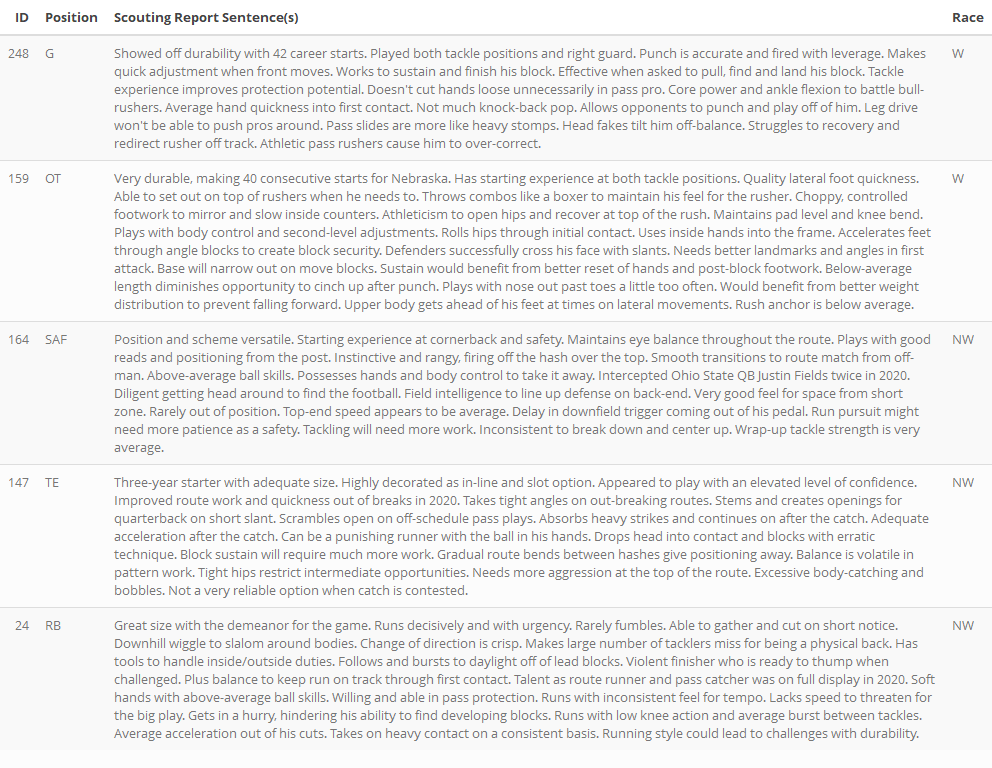
\includegraphics[width=1\linewidth]{Figures/all_sentence.png}
    \captionof{figure}{Random sample of Master dataset rows}
    \label{fig:master_dataset_sample}
  \end{minipage}%
\end{figure}
Some of this master dataset can be seen in \hyperref[fig:master_dataset_sample]{Figure 4.1}.
\subsection{1-Sentence Dataset}
This dataset is the master dataset split into 1-sentence rows. It consists of 4511 player rows. Of those rows, 3726 have been annotated as NW and 785 have been classed as W. An example of
this dataset can be seen below in \hyperref[fig:1-sentence_dataset_sample]{Figure 4.2}.

\begin{figure}[hb]
  \centering
  \begin{minipage}{1\textwidth}
    \centering
    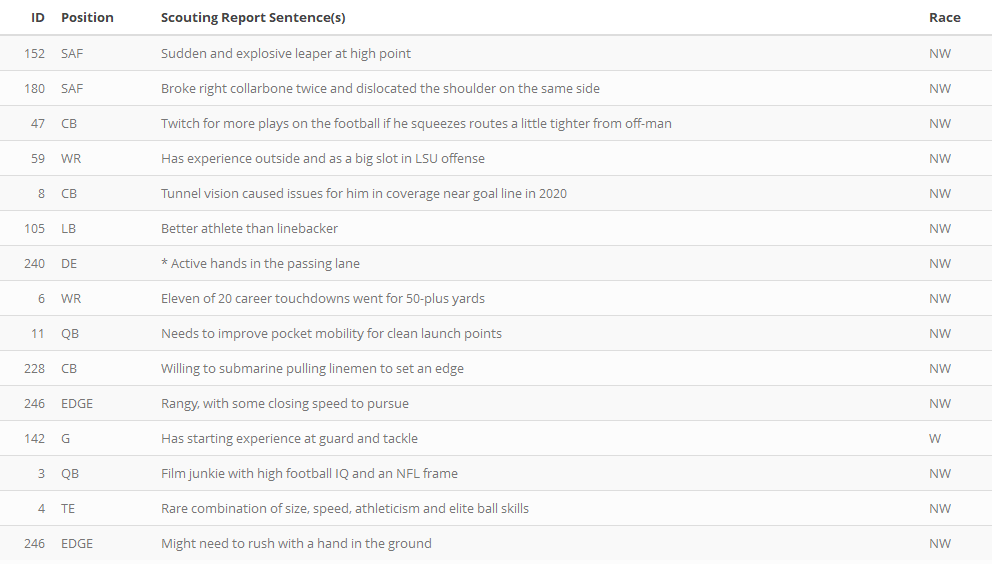
\includegraphics[width=1\linewidth]{Figures/1_sentence.png}
    \captionof{figure}{Random sample of 1-Sentence dataset rows}
    \label{fig:1-sentence_dataset_sample}
  \end{minipage}%
\end{figure}

\subsection{2-Sentence Dataset}
This data has also been garnered from the master dataset, with each row having 2 non-repeating sentences. As some players had a number of scouting report sentences not divisible by 2,
a random, previously seen sentence of theirs was randomly added to the data to complete that 2-sentence row. This was done by using modulo to get the sentences that needed supplementing.
There are 2448 rows in this dataset, 2022 of which are classified as NW and 426 as W. See \hyperref[fig:2-sentence_dataset_sample]{Figure 4.3} for a 2-Sentence data example.

\begin{figure}[htb]
  \centering
  \begin{minipage}{1\textwidth}
    \centering
    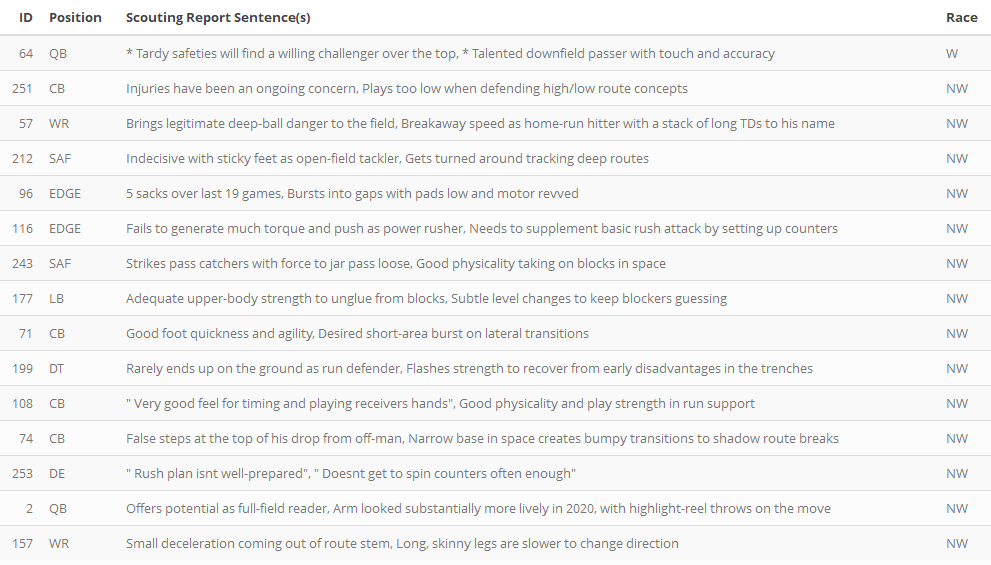
\includegraphics[width=1\linewidth]{Figures/2_sentence.png}
    \captionof{figure}{Random sample of 2-Sentence dataset rows}
    \label{fig:2-sentence_dataset_sample}
  \end{minipage}%
\end{figure}

\subsection{5-Sentence Dataset}
Similar to the 2-sentence dataset, this data was also pulled from the master dataset. Modulus was also used here to find rows lacking the 5 sentences needed. A random sample, the size of the need
of the row was taken from that players own pool of sentences. Steps were taken to ensure none of the sampled sentences were already part of the row in need. There are 1052 row in this dataset, 866 
of which have been classified as NW and 186 classed as W. An example of this dataset is below.

\begin{figure}[!htb]
  \centering
  \begin{minipage}{1\textwidth}
    \centering
    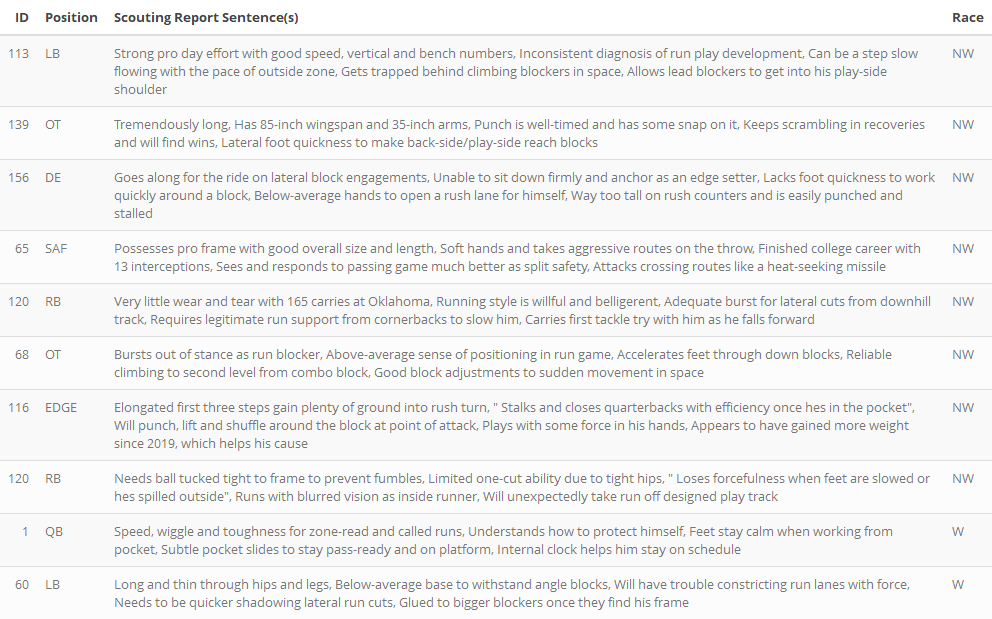
\includegraphics[width=1\linewidth]{Figures/5_sentence.png}
    \captionof{figure}{Random sample of 5-Sentence dataset rows}
    \label{fig:5-sentence_dataset_sample}
  \end{minipage}%
\end{figure}


\section{Sentiment Analysis Data}
\label{sec:senti_data}

\subsection{The GI dictionary}
The dataset which the Python GI dictionary helps create is GI tag comparison dataset. It consists of 4 columns:
\begin{itemize}
  \item Sentiment - A GI tag which appears at least once in the master dataset. There were 156 GI tags found in.
  \item \% of words with sentiment in white reports - The percentage of words that some GI tag is associated with in W reports.
  \item \% of words with sentiment in non-white reports - The percentage of words that some GI tag is associated with in NW reports.
  \item Relative \% difference - The relative difference in occurences of a GI tag in W and NW reports
\end{itemize}
From these 156 tags, 56 were deemed as relevant, a sample of which can be seen \hyperref[fig:GI_tag_comp]{Figure 4.5}.

\begin{figure}[!htb]
  \centering
  \begin{minipage}{1\textwidth}
    \centering
    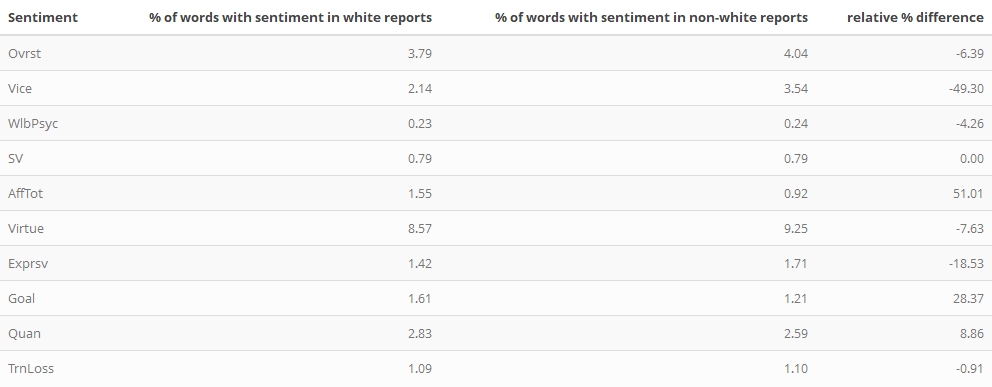
\includegraphics[width=1\linewidth]{Figures/enquirer.png}
    \captionof{figure}{Random 10 tag sample of GI tag comparison dataset}
    \label{fig:GI_tag_comp}
  \end{minipage}%
\end{figure}

\subsection{GI Tagged Dataset}
The GI tagged dataset is an almalgamation of the 1-Sentence dataset and the dataset filtered above. Given that one word can have many GI tags associated with it, this dataset contains
29137 rows. Each row has:
\begin{itemize}
  \item Sentence - The player report sentence in question.
  \item Tag - A GI tag associated with a word in that sentence.
  \item Race - The players ethnicity.
\end{itemize}
See \hyperref[fig:1-sentence_gi_tag_example]{Figure 4.5} for an example of a sentence that has multiple GI tags associated with it.
\begin{figure}[ht!b]
  \centering
  \begin{minipage}{1\textwidth}
    \centering
    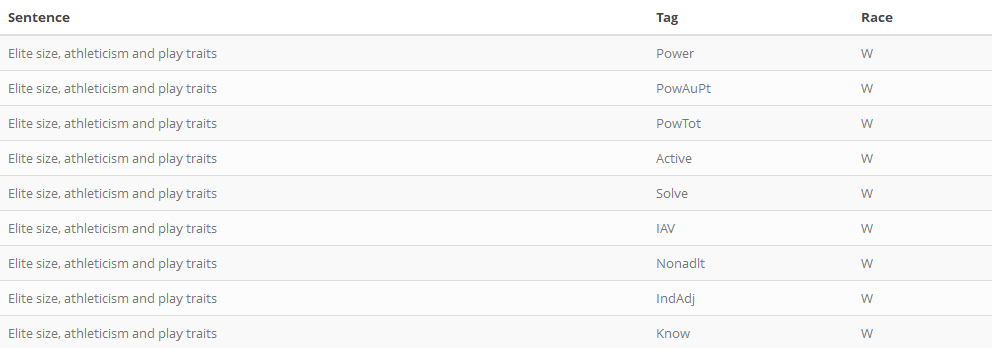
\includegraphics[width=1\linewidth]{Figures/1_sent_gi_tagged_specific.png}
    \captionof{figure}{Example of a sentence with multiple GI tags}
    \label{fig:1-sentence_gi_tag_example}
  \end{minipage}%
\end{figure}
This was the data used to perform sentiment analysis on a tag-by-tag basis.


\chapter{Experimental Settings}
\label{chap:experiments}
Described below is the complete experimental settings of the classification and sentiment analysis experiments. All experiments were completed using Python and the settings have been written 
to reflect this.
\section{Classification Settings}
The classification experiment is the most setting intensive of the 2 experiments. All 12 sentence datasets were used here. Following from the model desribed in \hyperref[chap:methodology]{Chapter 3},
the following settings were used to produce results. Before any experiments were run, text preprocessing was performed on the player report of the datasets that were read in:
\begin{itemize}
  \item With the NLTK library, stopword data was imported and set to 'english'.
  \item All punctuation was removed using the \texttt{string} library.
  \item Stemming was then done using NLTK's \texttt{PorterStemmer} function.
\end{itemize}
Each row of data was processed like this, the model extracting the processed player report and its label (W, NW). Scikit-learn's \texttt{{\it train{\_}test{\_}split}} function was then used to split the data into training
and test sets. This function had 2 settings, the train/test size split, which was set to 75/25, and \texttt{shuffle}, a boolean on whether or not to shuffle the data before splitting. This was assigned to \texttt{True}.
An instance of scikit-learn's \texttt{CountVectorizer} was then used. The function was given a ``strict'' setting in dealing with character it does not recognise. It was also set to also only vectorize unigrams. The vectorizer
was then trained on the training set features and applied to.
\subsection{Data Imbalance}
Data imbalance was corrected using imbalanced-learn's {\it Pipeline} classs. It requires a list of inputs to transform and sample the data. In this experiments case, the class was given a sampling strategy to resample all classes but the majority class,
and the ML algorithm to be used. Each ML algorithms settings are described in the \hyperref[sec:algor]{following subsection}.

\subsection{Algorithms}
\label{sec:algor}
Scikit-learn is used to implement all 4 ML algorithms used in this experiment. The library provides the ability to alter many aspects of each algorithm, so each algorithm's parameter were kept as default unless otherwise stated.
\begin{itemize}
  \item LR - This algorithm uses L2 regularization with a Limited-memory BGFS (Broyden-Fletcher-Goldfarb-Shanno) algorithm as its solver. The maximum amount of iterations for thes solver to converge has been set to 100.
  \item NB - The scikit-learn class \texttt{MultinomialNB} was used to implement the Naive Bayesian algorithm. This is because it is able to use the vectorization for text classification. The additive Laplace smoothing parameter was set to 1.
  \item SVM - The \texttt{SVC} (Support Vector Classification) class was used to imitate an SVM algorithm. A Radial Basis Function (RBF) was used as the kernel as it produced the best results. L2 regularization was also used.
  \item SGD - The SGD algorithm is implemented using the \texttt{SGDClassifier} class. The algorithms loss function was the hinge loss function. Again, L2 was the penalty used. The alpha value used was set to 0.0001. This was used to computer
              the learning rate as the learning rate parameter was set to ``optimal''. The training data for SDG was also shuffled after every epoch.
\end{itemize}
For each algorithm, the parameter \texttt{random\_state} was set to a constant integer number, for result reproducability.
\subsection{Evaluation}
10-fold cross validation was implemented using the \texttt{RepeatedStratifiedFold} class. 10 splits were specified for the number of folds. 3 cross-validator repeats were also specified. Score evaluation was then done through the \texttt{cross\_val\_score}
function. This used the pipeline built, and accepted a data list of the sentences to classify and the data list of player race as its target variable. 2 scoring metrics were recorded, algorithm \texttt{accuracy} and algorithm \texttt{f1-score}. These scoring functions
were passed into the \texttt{cross\_validate} evaluator. The result was the mean of the 10 scores, 1 from each of the folds performed. Experiment results and analysis is discussed in \hyperref[chap:results]{Chapter 6}.

\section{Sentiment Analysis Settings}
The sentiment analysis experiment uses a Python implementation of the Harvard GI dictionary, its creation discussed here. The \texttt{pysentiment2} \footnote{\url{https://pypi.org/project/pysentiment2/}} library was used to tokenize each player report column in each row. This library was used over other tokenization
methods as it contains the Harvard GI dictionary as its library, an instance of which can be called for the purpose of tokenization. This was used to tokenize every player report sentence in the 1-sentence dataset, an example of which can be seen in  \hyperref[fig:1-sentence_gi_tag_example]{Figure 4.4}. \par
This dataset, along with the maunually filtered GI tags list, is the input to the model that gets the average sentiment for each GI tag for all W and NW sentences associated with that tag. Each row in the dataset is read and the sentence's polarity calculated using \texttt{pysentiment2}'s tokenization and sentiment score
functions. These functions were used in their default settings. The model then adds this polarity score to either the W polarity score or the NW polarity score. Once the dataset has been iterated through, it outputs the average W and NW polarity for the GI tag in question, as well as the difference between the two polarities. 
The model produces this result for every GI tag it is given.

\chapter{Results}
\label{chap:results}
Results first, using figures and tables, with little commentary and no interpretation.
Then analysis and interpretation.
The results chapter presents the findings from both experiments described in the Methodology and Experiments chapters.
\section{Classification}
This section presents results in relation to the classification experiment. Overall, 12 different datasets were passed through the model, totaling 96 outputted results between the accuracy and f1-score. 
Both higher accuracy and F1-Score indicates better performance of the algorithm. From our results we can interpret how much information different algorithms need to produce the best results possible.\par

\subsection{1-Sentence Results}
\begin{table}[!h]
  \begin{adjustbox}{center,max width=\linewidth}
    \begin{tabular}{l|cccc}
      \toprule
      \bf Algorithm & \bf \stackbox[c]{Raw Sentences} & \bf \stackbox[c]{GI Tagged\\ Sentences}& \bf \stackbox[c]{Binary-GI \\Sentences}  \\
      \midrule
      Logistic Regression         & 0.71         & 0.645         & 0.565                \\
      Naive Bayes                 & 0.681        & 0.628         & 0.579                \\
      Support Vector Machine      & 0.806        & 0.723         & 0.682                \\
      Stochastic Gradient Descent & 0.706        & 0.636         & 0.562                \\
    \bottomrule
    \end{tabular}
  \end{adjustbox}
  \caption{1-Sentence Classification Accuracy}
  \label{tab:1S_accuracy}
\end{table}

\begin{table}[!h]
  \begin{adjustbox}{center,max width=\linewidth}
    \begin{tabular}{l|cccc}
      \toprule
      \bf Algorithm & \bf \stackbox[c]{Raw Sentences} & \bf \stackbox[c]{GI Tagged\\ Sentences}& \bf \stackbox[c]{Binary-GI \\Sentences} \\
      \midrule
      Logistic Regression             & 0.313        & 0.27         & 0.301              \\
      Naive Bayes                     & 0.339        & 0.286        & 0.291              \\
      Support Vector Machine          & 0.181        & 0.239        & 0.251              \\
      Stochastic Gradient Descent     & 0.294        & 0.261        & 0.284              \\
    \bottomrule
    \end{tabular}
  \end{adjustbox}
  \caption{1-Sentence Classification F1-Scores}
  \label{tab:1S_f1}
\end{table}

In the context of the 1-Sentence datasets, Table 6.1 shows that the SVM algorithm produced the best classification accuracy results across all 3 different dataset types. LR, NB, and SGD all had similar scores
across the 3 dataset types. Overall, the raw sentences version of the 1-Sentence dataset gave the highest accuracy, with the GI Tagged 1-Sentence giving the 2nd highest results. \par
The NB algorithm gave the single highest F1-score, and was consistently high overall. Again, SGD and LR shared similar results. SVM produced the worst F1-Scores in Table 6.2 for each of the 3 dataset types.

\subsection{2-Sentence Results}
\begin{table}[!h]
  \begin{adjustbox}{center,max width=\linewidth}
    \begin{tabular}{l|cccc}
      \toprule
      \bf Algorithm & \bf \stackbox[l]{Raw Sentences} & \bf \stackbox[c]{GI Tagged\\ Sentences}& \bf \stackbox[c]{Binary-GI \\Sentences}  \\
      \midrule
      Logistic Regression         & 0.754        & 0.691         & 0.603                \\
      Naive Bayes                 & 0.746        & 0.675         & 0.603             \\
      Support Vector Machine      & 0.83         & 0.77          & 0.738          \\
      Stochastic Gradient Descent & 0.759        & 0.689         & 0.616               \\
    \bottomrule
    \end{tabular}
  \end{adjustbox}
  \caption{2-Sentence Classification Accuracy}
  \label{tab:2S_accuracy}
\end{table}

\begin{table}[!h]
  \begin{adjustbox}{center,max width=\linewidth}
    \begin{tabular}{l|cccc}
      \toprule
      \bf Algorithm & \bf \stackbox[l]{Raw Sentences} & \bf \stackbox[c]{GI Tagged\\ Sentences}& \bf \stackbox[c]{Binary-GI \\Sentences} \\
      \midrule
      Logistic Regression             & 0.333       & 0.257         & 0.311                  \\
      Naive Bayes                     & 0.396       & 0.293         & 0.3                \\
      Support Vector Machine          & 0.19        & 0.218         & 0.253                  \\
      Stochastic Gradient Descent     & 0.308       & 0.246         & 0.294                 \\
    \bottomrule
    \end{tabular}
  \end{adjustbox}
  \caption{2-Sentence Classification F1-Scores}
  \label{tab:2S_f1}
\end{table}

From Table 6.3, again the SVM algorithm has the best accuracy results, in this case for the 2-Sentence datasets. Each of the other 3 algorithms scored similarily
in each of the 3 dataset types. The raw sentence dataset type produced the highest accuracy in all 4 machine learning algorithms. The Binary-GI tagged
sentences had the worst accuracy performance for each algorithm.\par
Table 6.4 indicates that the NB algorithm produced the highest F1-Scores in the Raw Sentences and GI Tagged Sentences datasets. LR and SGD had similar results here too. SVM produced the
lowest F1-Scores in each dataset type. Like the 1-Sentence dataset, the raw sentences dataset type performed the best.

\subsection{5-Sentence Results}

\begin{table}[!h]
  \begin{adjustbox}{center,max width=\linewidth}
    \begin{tabular}{l|cccc}
      \toprule
      \bf Algorithm & \bf \stackbox[l]{Raw Sentences} & \bf \stackbox[c]{GI Tagged\\ Sentences}& \bf \stackbox[c]{Binary-GI \\Sentences}  \\
      \midrule
      Logistic Regression         & 0.816        & 0.732         & 0.723                \\
      Naive Bayes                 & 0.833        & 0.739         & 0.686             \\
      Support Vector Machine      & 0.842        & 0.742         & 0.771          \\
      Stochastic Gradient Descent & 0.816        & 0.738         & 0.735               \\
    \bottomrule
    \end{tabular}
  \end{adjustbox}
  \caption{5-Sentence Classification Accuracy}
  \label{tab:5S_accuracy}
\end{table}

\begin{table}[!h]
  \begin{adjustbox}{center,max width=\linewidth}
    \begin{tabular}{l|cccc}
      \toprule
      \bf Algorithm & \bf \stackbox[l]{Raw Sentences} & \bf \stackbox[c]{GI Tagged\\ Sentences}& \bf \stackbox[c]{Binary-GI \\Sentences} \\
      \midrule
      Logistic Regression             & 0.459       & 0.285          & 0.32                  \\
      Naive Bayes                     & 0.55        & 0.312          & 0.328                \\
      Support Vector Machine          & 0.253       & 0.242          & 0.249                  \\
      Stochastic Gradient Descent     & 0.399       & 0.263          & 0.298                 \\
    \bottomrule
    \end{tabular}
  \end{adjustbox}
  \caption{5-Sentence Classification F1-Scores}
  \label{tab:5S_f1}
\end{table}

From Table 6.5, it can be seen that all 4 algorithms performed well on the raw sentences dataset, each scoring over 80\% accuracy. SVM and NB had the
highest results overall, though all 4 algorithms scored similarily. Raw Sentences again had the highest accuracy, with the GI Tagged and Binary-GI sentences
reporting similar accuracy results for each of the algorithms used.  \par
In Table 6.6, NB has the best F1-score in all of the 5-Sentence dataset types, followed by LR. In the 5-sentence experiment, a clear separation can be seen between 
the 4 machine learning algorithms. The Binary-GI dataset outperformed the GI Tagged dataset here. SVM performed the worst of the 4 algorithms in each dataset type.

\subsection{All Sentence Results}

\begin{table}[!h]
  \begin{adjustbox}{center,max width=\linewidth}
    \begin{tabular}{l|cccc}
      \toprule
      \bf Algorithm & \bf \stackbox[l]{Raw Sentences} & \bf \stackbox[c]{GI Tagged\\ Sentences}& \bf \stackbox[c]{Binary-GI \\Sentences}  \\
      \midrule
      Logistic Regression         & 0.824         & 0.774         & 0.723                \\
      Naive Bayes                 & 0.829        & 0.829          & 0.686             \\
      Support Vector Machine      & 0.828        & 0.781          & 0.771          \\
      Stochastic Gradient Descent & 0.828        & 0.787          & 0.735               \\
    \bottomrule
    \end{tabular}
  \end{adjustbox}
  \caption{All-Sentence Classification Accuracy}
  \label{tab:All_S_accuracy}
\end{table}

\begin{table}[!h]
  \begin{adjustbox}{center,max width=\linewidth}
    \begin{tabular}{l|cccc}
      \toprule
      \bf Algorithm & \bf \stackbox[l]{Raw Sentences} & \bf \stackbox[c]{GI Tagged\\ Sentences}& \bf \stackbox[c]{Binary-GI \\Sentences} \\
      \midrule
      Logistic Regression             & 0.431        & 0.266         & 0.304                  \\
      Naive Bayes                     & 0.457        & 0.28          & 0.262                \\
      Support Vector Machine          & 0.047        & 0.405         & 0.169                  \\
      Stochastic Gradient Descent     & 0.391        & 0.261         & 0.261                 \\
    \bottomrule
    \end{tabular}
  \end{adjustbox}
  \caption{All-Sentence Classification F1-Scores}
  \label{tab:All_S_f1}
\end{table}

In Table 6.7, it can be seen that all 4 algorithms performed very similarily on the all-sentence \footnote{The all-sentence datasets is the master dataset, the master dataset GI Tagged and Binary-GI'ed}, 
raw sentences dataset type. NB had the highest accuracy for the GI Tagged dataset and the lowest accuracy on the Binary-GI dataset type. LR and SGD had similar accuracy across all dataset types. The raw sentence
dataset type lent itself to providing the highest accuracy. Binary-GI produced slightly worse accuracy results than GI Tagged. \par
Table 6.8 shows that the NB algorithm produced the best F1-Score for Raw Sentences, SVM produced the highest F1-Score for the GI Tagged sentences, and LR the highest for Binary-GI. SVM produced poor results
for both Raw Sentences and Binary-GI. As a whole, Raw Sentences provided the highest F1-Scores, while GI Tagged and Binary-GI gave similar scores.


\subsection{Results Interpretation}
From the results of each of the 4 (1-Sentence, 2-Sentence, 5-Sentence, All-Sentence) sentence level experiments, several interpretations can be made, firstly with regards to accuracy:
\begin{itemize}
  \item Of the 3 dataset types (Raw Sentences, GI Tagged, Binary-GI) it is clear that the Raw Sentences version of each of the 4 sentence levels produced the highest accuracy, regardless of what algorithm was used. The Raw
        Sentences 4 gave a mean accuracy of 78.8\%, with GI Tagged and Binary-GI only achieving accuracy levels of 72.3\% and 65.7\% respectively.
  \item The SVM algorithm stood out as having the highest accuracy overall, with the algorithm averaging an accuracy of 77.2\% across all dataset types and sentence levels. The other 3 algorithms varied in their
         accuracy standings across the 4 sentence levels, but had extremely similar average accuracy with, SGD averaging 70.8\%, LR averaging 70.7\%, and NB averaging 70.6\%.
  \item Another result we can extrapolate from the tables shown is the accuracy on a sentence level to sentence level basis across the 3 dataset types. The 1-Sentence, 2-Sentence, 5-Sentence, All-Sentence dataset had an average
        accuracy of 66\%, 70.6\%, 74.4\%, and 78.3\% respectively. This shows that the more data in the scouting report available to each algorithm, the better it can classify the player.
\end{itemize} 

The F1-Score results shall also be discussed. One generic finding from the F1-Score is that LR, NB, and SGD had a higher recall metric score than precision score. The SVM F1-Scores always produced a balance of the two metrics. 
Several more interpretations can be made from the F1-Score results:
\begin{itemize}
  \item Like the accuracy results, the Raw Sentence version of each of the 4 sentence levels gave the highest F1-Score in comparison to GI tagged and Binary-GI, achieving an average F1-Score of 0.34, compared to GI tagged's 0.27 
         and Binary-GI's 0.28. Binary-GI's F1-Score being similar to GI Tagged was unexpected given that GI Tagged far outperforms Binary-GI in terms of accuracy.
  \item The NB algorithm had the highest average F1-Score across all dataset types and sentence levels, with a score of 0.34,. LR was second best in this respect,
        averaging 0.32. SGD averaged 0.30. SVM performed by far the worst, averaging only 0.22. This is due to the fact that the other 3 algorithms recall was much higher than SVM's at every sentence level with every dataset type.
  \item Finally, the 5-Sentence type had the highest average F1-Score of the 4 sentence levels, averaging 0.33. The 1-Sentence, 2-Sentence and All-Sentence were bunched together in terms of score, achieving an average of 0.28, 0.28, and
        0.29 respectively. This means that the NB algorithm on the 5-Sentence Raw Sentence dataset had the best individual score with 0.55.
\end{itemize}

Overall, this experiment showed that the Raw Sentence type was the best for text classification regardless of sentence level. This is because of how well the word vectorizer works with sentence data. It also showed that the Binary-GI was the worst
dataset type for classification. This is due to the sparse nature of the dataset, as only a 5 to 10 columns would be set to 1 on each row. The number of features was also a cause of low performance, as the dataset had 156 features, 1 feature for every 
GI Tag found in all the data. Something interesting from these results was the difference in result order of the algorithms between accuracy and F1-score. Accuracy results went: SVM with the highest average, then SGD, then LR, then NB. F1-Scores was the 
reverse of this: NB producing the highest, LR, SGD, and SVM following in that order. One of the reasons is because of NB, LR, and SGD's high recall metrics. High precision was the reason SVM was able to achieve such high accuracy. \par
From the classification accuracy produced in this paper, it can be concluded that \textbf{W} and \textbf{NW} players can be classified to a high degree of accuracy using machine learning methods of text classification. 

\section{Sentiment Analysis}

\subsection{Experiment Results}
figs and tables


\subsection{Interpretation}
Remember to show examples

\chapter{Conclusion}
\label{chap:conclusion}
Here you must zoom back out to evaluate the thesis. Mention limitations and weaknesses as well as contributions.

\section{Thesis Evaluation}
What i wanted to do, and what i learned
\subsection{Contributions}
datasets created, 1,2,5 and 1-GI tagged. showed ML strengths.  
\subsection{Weaknesses}
what is a significant difference for sentiment analysis score?
dataset small as oversampling needed.
No DeepL methods for classification.
choosing GI tags when filtering
\section{Future Work}
DeepL methods for classification.
Classify on GI tags of sentences
bigger dataset

%%%%%%%%%%%%%%%%%%%%%%%%%%%%%%%%%%%%%%%%%%%%%%%%%%%%%%%%%%%%%%%%%%%%%%%%%%%%%%%%
\bibliographystyle{plainnat}                  % to give author-year style
\renewcommand{\bibname}{References}           % change default name Bibliography to References
\bibliography{references}                     % References file, references.bib
\addcontentsline{toc}{chapter}{References}    % add References to TOC


%%% uncomment if Appendix needed
\appendix
\chapter{Code} 
\label{chap:Code}
See \href{https://github.com/EoghanOGallchoir/Thesis_Code}{GitHub repository} for thesis code and data (repo currently private).


\end{document}
